\documentclass{iitthesis}


% Document Options:
%
% Note if you want to save paper when printing drafts,
% replace the above line by
%
%   \documentclass[draft]{iitthesis}
%
% See Help file for more about options.

\usepackage{graphicx}    % This package is used for Figures

\begin{document}

%%% Declarations for Title Page %%%
\title{Acceptance of Code Contributors on GitHub}
\author{Matthew Heston}
\degree{Master of Science}
\dept{Information Architecture}
\date{May 2014}
% \copyrightnoticetrue      % crate copyright page or not
%\coadvisortrue           % add co-advisor. activate it by removing % symbol to add co-advisor
\maketitle                % create title and copyright pages


\prelimpages         % Settings of preliminary pages are done with \prelimpages command


%%%  Acknowledgement %%%
\begin{acknowledgement}     % acknowledgement environment, this is optional
\par  This dissertation could not have been written without Dr. X
who not only served as my supervisor but also encouraged and
challenged me throughout my academic program. He and the other
faculty members, Dr. Y and Dr. Z, guided me through the
dissertation process, never accepting less than my best efforts. I
thank them all.\\ \\ (Don't copy this sample text. Write your own
acknowledgement.)
% or \input{acknowledgement.tex} % you need a separate acknowledgement.tex file to include it.
\end{acknowledgement}


% Table of Contents
\tableofcontents
\clearpage

% List of Tables
\listoftables

\clearpage

%List of Figures
\listoffigures

\clearpage

%List of Symbols(optional)

% \listofsymbols
%  \SymbolDefinition{$\beta$}{probability of non-detecting bad data}
%  \SymbolDefinition{$\delta$}{Transition Coefficient Constant for the Design of Linear-Phase FIR Filters}
%  \SymbolDefinition{$\zeta$}{Reflection Coefficient Parameter}


%  \clearpage



%%% Abstract %%%
\begin{abstract}           % abstract environment, this is optional
\par Your Abstract goes here!
% or \input{abstract.tex}  %you need a separate abstract.tex file to include it.
\end{abstract}


\textpages     % Settings of text-pages are done with \textpages command

% Chapters are created with \Chapter{title} command
\Chapter{INTRODUCTION}

% Section are created with \Section{title} command
\Section{GitHub} \label{sec:github}
GitHub is a social website that open source software developers use to host
their software projects and to browse other developers' projects. It includes
many features that are present on social networking sites, such as the ability
to follow other users and leave comments on projects. In the study of computer
supported cooperative work, GitHub provides a wealth of data, as it is a
centralized location where many different tasks take place. For example, users
can create bug reports, submit fixes, and engage in discussions about new
features all on one website.  In this study, we use statistical and machine
learning methods on data from GitHub repositories to explore how different
social factors may affect the acceptance of code changes from first time
contributors.

\Section{Related Work}
GitHub itself has not been extensively studied. ~\cite{choi_herding_2013} use
data from the website to examine what they call \textit{herding behavior} of
developers in open source projects.  ~\cite{mcdonald_performance_2013} provide a
qualitative exploratory study on how developers on the website measure success
of projects. Of importance to our study is their findings that developers
believe the GitHub interface has changed the way developers are able to
participate in the community. While they describe how features of the website
are used by developers to measure community involvement and activity, we are
concerned with how these features can provide measures that insight into how
contributions by new community members are accepted by core members.

While there are not many studies on GitHub itself, there are many studies that
explore different open source communities. These include theoretical
perspectives on knowledge building and success in open source
projects~\cite{hemetsberger_learning_2006}~\cite{hemetsberger_collective_2009}
and the motivations of open source
developers~\cite{hertel_motivation_2003}\cite{lakhani_why_2003}.

Our study seeks to which factors contribute to the acceptance of code
contributions of first time contributors. We draw on findings from previous
studies that describe the joining process of new developers
~\cite{huang_mining_2005}\cite{von_krogh_community_2003}. We also draw from work
that describes joining processes not only in open source software, but also from
other computer mediated collaborative contexts, such as
Wikipedia~\cite{bryant_becoming_2005}. Our goal is to provide an empirical
understanding of community acceptance on a relatively new social platform.


The remainder of this article is organized as follows.
Section~\ref{data} begins with a description of some of the terminology specific
to GitHub, since many of the features in our models rely on an understanding of
this terminology. We then describe how we measured various social factors and
present our hypotheses. In Section~\ref{methods} we describe our experiments. We
find that the variables we chose lack predictive power of pull request
acceptance. Section~\ref{discussion} describes why our models may have failed
and presents some observations from the data. Finally, Section~\ref{conclusion}
presents our conclusions and ideas for future work.

\Chapter{DATA}

\Section{Terminology} \label{sec:terms}
A software project on the website is referred to as a \textit{repository}. Any
user on GitHub can \textit{star} a repository. Users star repositories to be
able to easily navigate to it and to receieve updates on activity from the
repository. If a developer wants to contribute to another one of developer's
repositories, he can \textit{fork} the repository, which creates a copy of the
project for him to work on. As the developer makes changes to this code, he
\textit{commits} his changes. A \textit{commit} is a snapshot of the code at a
certain point in time. When the developer is finished, he can submit a
\textit{pull request} to the owner of the project. All pull requests for a
project are viewable on GitHub, and any user of the site can comment on them. A
pull request can have a status of open or closed. A status of open indicates
that that owner of the repository has not made a decision about whether or not
to include the changes. If the owner of a repository wants to incorporate the
changes the developer made, he can \textit{merge} them into the repository. A
pull request can be closed without being merged, which means that the changes
the developer made were not accepted.

\Section{Data Collection}
Data was collected using the GitHub API.\footnote{http://developer.github.com/}
We collected pull requests from 45 different repositories. The repositories
selected came from the top 100 most starred repositories on GitHub. We chose
popular repositories with the assumption that they would be maintained by an
active community. We only consider pull requests with a status of closed. This
resulted in approximately 44,400 pull requests. For most of our experiments, we
will use what we refer to as first pull requests, by which we mean the first
pull request a user submitted to a repository. Filtering for these pull requests
results in a sample size of 13,383. To find merged pull requests, we first
filter all pull requests that are marked as merged by the GitHub API, meaning
that the project maintainers used GitHub's merge feature to accept the pull
request. In some repositories, project maintainers use a different workflow when
accepting pull requests, wherein the code changes are accepted, but it is not
reflected as merged on GitHub. In most of these cases, there is a standard way
of reflecting this in the commit comments, so we use some naive heuristics for
identifying these requests by searching commit comments for certain text
patterns. This results in 5,239, or 39.1\% of first pull requests being merged.

\Chapter{METHODS}

\Section{Communities of Practice}
~\cite{lave_situated_1991} describe learning in communities of practice as
taking place through a process of \textit{legitimate peripheral participation},
wherein newcomers join a community by participating in peripheral tasks and
forming relationships to move towards the center of the community. This concept
has been explored in many studies of computer mediated communication.  In their
study on members of Wikipedia, ~\cite{bryant_becoming_2005} note that members
initially become involved through peripheral activities. These are simple and
low risk activities members can take part in to learn more about the community
before trying to become major contributors. Similarly,
~\cite{von_krogh_community_2003} from observing open source communities generate
the construct of a \textit{joining script}, where each project has a set of
tasks for new developers to go through before being accepted into the community.
In a discussion of successful developers on the Python project,
~\cite{ducheneaut_socialization_2005} describe the first steps of their
trajectory as including peripheral monitoring of development activity and
reporting of bugs.

We consider the main peripheral activity a user can participate in on GitHub is
commenting on other pull requests. For each first pull request in our dataset,
we count the number of other pull requests the user commented on before
submitting. Based on the these previous findings, we would expect to see a
positive correlation between this number and the likelihood that a pull request
is recieved. We also count the number of comments that each first pull request
recieves, with the assumption that this variable can be used to measure the
amount of community interest in a given pull request. We plot these variables in
Figure~\ref{fig:aprr_up}.

\Subsection{User Participation}
We see that user participation for the majority of all first pull requests, both
merged and not merged, is 0. This indicates that in general, most users are not
attempting to engage in the peripheral activity of commenting on other pull
requests before submitting their own. The GitHub interface makes it relatively
easy for a user to fork a repository, make changes, and submit the changes for
consideration. Previous studies on GitHub have shown that the number of
contributions did increase for some projects that moved from other hosting
options to GitHub~\cite{mcdonald_performance_2013}. It is possible this
interface lowers the barrier of entry for a developer who wants to contribute to
a project, and allows them to bypass participating in the joining script
described by ~\cite{von_krogh_community_2003}.

We also examine these variables for first pull requests by users who later
submit another pull request. Our intuition here is that some users might
encounter a bug they fix or desire a feature that they implement, and then
submit these changes back to repository. They may not comment on other pull
requests as they are not interested in becoming long term members of the
community, but rather are just interested in submitting a one time patch.
Figure~\ref{fig:aprr_up_repeaters} shows a visualization of the same first pull
requests, but only for users who submit at least one other pull request at a
later point in our data set, and Figure~\ref{fig:aprr_up_repeaters_5} shows the
data for users who submit at least 10 more times. Looking at users who submit
at least one other time cuts our number of observations from 13,383 to 5,207,
indicating that approximately 61\% of these pull requests come from users who
will not contribute any others. Looking at users who will submit at least 10
more times gives us a total of 1,155 observations.

It is clear that in all these cases, regardless of whether or not they will be
continuing to submit other pull requests later, at the time of submitting their
first pull request, users are generally not participating in the community. The
previous graphs only consider the number of pull requests a user commented on
before submitting their first pull request, so we do not capture how users who
submit multiple pull request over time comment on other pull requests over time.
In Figure~\ref{fig:commented_pullrequests_totals} we plot the total number of
others' pull requests that a user commented on by how many pull requests they
submitted themselves, considering only users who have submitted at least two
pull requests. There is not a strong correlation between these variables
(Spearman's $\rho$  = 0.44), indicating that users do not necessarily
participate in more commenting as they continue to submit more pull requests.

\begin{figure}[p] \centering \label{fig:aprr_up}
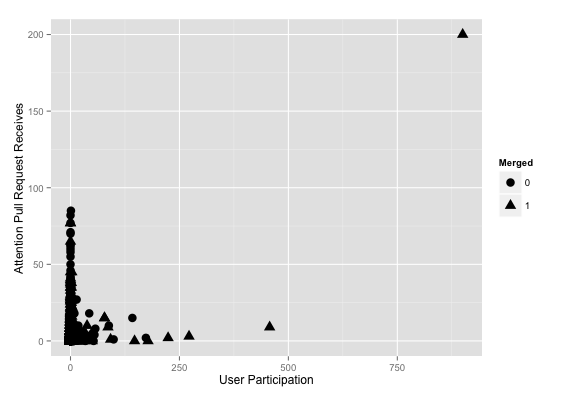
\includegraphics[scale=0.6]{figures/aprr_up_ggplot.png} \caption{User
participation and attention a pull request recieves for all first pull
requests.} \end{figure}

\begin{figure}[p] \centering \label{fig:aprr_up_repeaters}
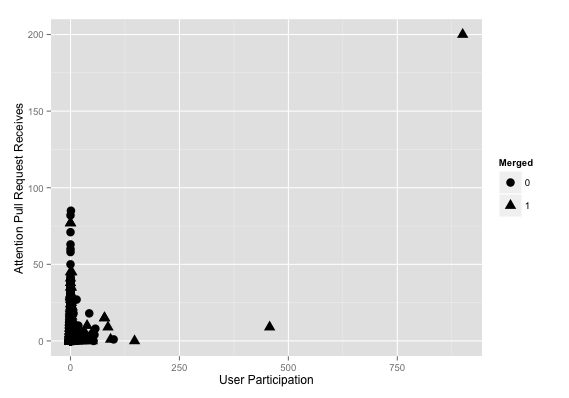
\includegraphics[scale=0.6]{figures/aprr_up_repeaters_ggplot.png} \caption{User
participation and attention a pull request recieves variables for users who
submit at least one other pull request in our data set.} \end{figure}

\begin{figure}[p] \centering \label{fig:aprr_up_repeaters_10}
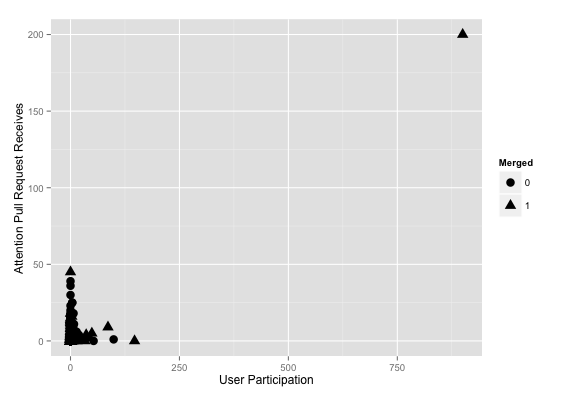
\includegraphics[scale=0.6]{figures/aprr_up_repeaters_10_ggplot.png}
\caption{User participation and attention a pull request recieves variables for
users who submit at least 10 other pull requests in our data set.} \end{figure}

\begin{figure}[p] \centering \label{fig:commented_pullrequests_totals}
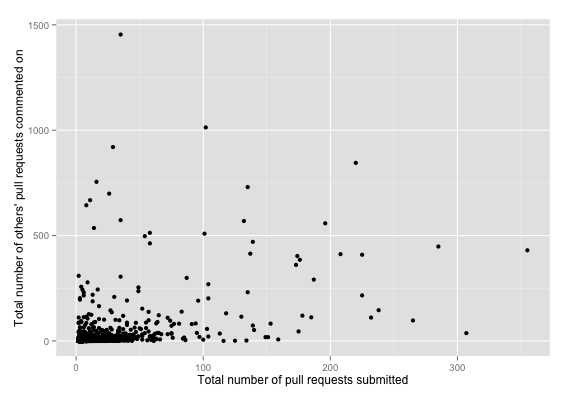
\includegraphics[scale=0.6]{figures/commented_pullrequests_totals_ggplot.png}
\caption{Total number of pull requests commented on and total number of pull
requests submitted for each user.} \end{figure}

\Subsection{Attention Pull Request Receives}
In Figure~\ref{fig:aprr_up}, we see more variance in the number of comments on
first pull requests than we did with the number of pull requests users commented
on before submitting. However, there is clearly no linear separation of merged
and not merged pull requests using this variable, so it seems just viewing the
amount of activity a pull request receives is not enough to explain whether or
not it gets merged.

To test whether or not the content of these comments is predictive of whether or
not a pull request is merged, we collect the comments for each of our first pull
requests. We ignore comments made by the user who submitted the pull request,
since we are interested in what other users had to say about it. We also ignore
the last comment associated with a pull request, since these often will
explicitly say whether or not the maintainer is merging the pull request or not.
We are more interested in if the type of language used in the discussion of a
pull request is predictive of whether or not it is accepted. We ignore pull
requests that only have one comment associated with it. This gives us a sample
size of 5,674. 3,811, approximately 67\% are unmerged. We treat the remaining
comments associated with the pull request as one document, and convert them into
feature vectors representing the count of each unigram and bigram in the
documents, and train both a logistic regression and naive bayes classifier using
this feature set. The results of testing these classifiers is shown in
Table~\ref{tbl:classifiers}. The results shown are the result of running 10-fold
cross validation. The low recall rates indicate that data we have is not
sufficient to distinguish positive cases. Of course, our sample size of 5,674 is
relatively small, but it is interesting to note that only 42\% of the first pull
requests in our data set have more than 1 comment associated with them.

\begin{table} \centering \label{tbl:classifiers}
  \begin{tabular}{lll}
  ~         & Logistic Regression & Naive Bayes \\
  Accuracy  & 69.6\%              & 70.6\%      \\
  Precision & 56.0\%              & 60.3\%      \\
  Recall    & 36.1\%              & 30.7\%      \\
  \end{tabular}
\end{table}



\Section{First Mover Advantage}
~\cite{viegas_studying_2004} find what they call a \textit{first-mover
advantage} in the editing of Wikipedia articles, wherein the first contribution
to a page tends to survive longer and recieve less modifications than following
contributions.


\clearpage


%
% APPENDIX
%

% Do the settings of appendices with \appendix command
\appendix

% Then create each appendix using
% \Appendix{title_of_appendix} command
%
% BIBLIOGRAPHY
%
% you have two options: 1) create bibliography manually,
% 2) create bibliography automatically. See BibliographyHelp.pdf file for details.


\bibliographystyle{plain}
\bibliography{Master}

\end{document}  % end of document
